
\section{Introduction}

In this chapter, we will sample on BTCUSD and BTCUSDT dataset across all features and more specifically volume, side of the trade, speed of the market, and convergence of exchanges in various features. For simplicity reasons, when sampling takes place on all exchanges, the dataset will be aggregated to the 'second' or 'minute' interval (the 'minute' interval sampling will be used mostly for plotting purposes). In other occasions, the sampling will take place directly on raw tick data, nevertheless, in order to create the dataset for all exchanges, some sort of aggregation must be used, mostly with respect to time.

\section{Volume}

In this section, we will use volume along with different features of choice such as, positive-negative returns and buying-selling. We will begin with buying-selling volume, while we illustrate how the sampling could end up in signal creation.

\subsubsection{Buying and Selling Volume}

The dataset on which the next sampling is performed, is created by classifying the volume into buying and selling volume, depending on who initiated the trade (bid or ask). This classification is taking place directly on tick data. Then, the dataset is aggregated (summation) on the 'second' time interval, where two columns are created: one for the buying volume and one for the selling volume. This procedure is used for all exchanges and as we have shown, all exchanges should be used (see \ref{fig:cum}). 

The latter results to a 10 column dataset where 5 columns are created for the buying volume and 5 columns for the selling volume (two columns for each exchange). Lastly, the 5 columns of each side, are summed row-wise in order to create one column for buy and one column for sell. The last columns represent the volume that took place on all exchanges after being classified as buying and selling.

In order to model the two volumes, we will use a Hawkes process. To provide the reader with a brief explanation of the Hawkes process, we shall begin with a Poisson process, which models the number of occurences at certain time intervals. The key takeaways from Poisson processes are that the expected rate of these occurrences \( \lambda \) is stable (homogeneity) and that the expected rate of occurrences at a future time interval is independent of past occurrences. 

In order to study more complex phenomena, a Non-homogeneous Poisson process could be used, where the future events are still independent of past phenomena, but \( \lambda \) is now a function of time. This particular idea fits somewhat with market behavior, in that the expected rate of returns (or as we will later show), the expected rate of volume traded, does seemingly not behave independently of the time interval, but fluctuates locally. There are certain periods of time where the volume that is expected to be traded is higher (moments of behavior co-ordination). For the function \( \lambda(t) \) to be called a deterministic function (and also non-homogeneous Poisson process) there are certain axioms that need to be held. This function then is called an “Intensity function”.

Lastly, in addition to the above, if the intensity function is not stable, but is affected by the history of the timeseries up to time \(t\), the process is called Hawkes process. A Hawkes process is a self-exciting process, which its past events affect the current value of the process. There also exist other similar approaches to Hawkes, such as convolutional neural networks which are mostly used for image classification that use a weighted average of previous values. The problem with this approach, contrary to Hawkes is that this approach would enforce static dependencies while Hawkes intensity function uses the \(N(t)\) counting process as a positive reinforcement that decays exponentially in such a way that past events that are close to time \(t\), affect the value of the function much more than, say older events that are further away from \(t\) \cite{hawkes2}. 

In a volume specific example the formula would be:
\[ \lambda(t|H_t) = \lambda_0(0|H_0) + \sum_{i=1}^{N(t)}\text{Vol}(i) \cdot e^{-\delta(t-T_i)} \]
where \(\lambda_0(0|H_0) \) is the initial intensity and \( \delta \) would be a positive dampening coefficient that implies the rate at which the function decays.

Using a Hawkes process with \( \delta = 0.2 \) and \( \lambda_0 = 0 \), we modeled the buy and sell volume, and upon the new dataset, we sampled using two parallel moving averages, one slow (larger scope) and one faster (smaller window). The sampling took place, when the fast MA exceeded the slow MA by a threshold. This way, we can have an overview of the buying and selling volume surges. First thing to notice, is that most of the points sampled from the two volumes are different (see \ref{fig:hawkes1}). There is an oversampling in sudden price action and no sampling at all when price goes sideways. Furthermore, the buying volume, is found mostly in local maxima and the selling volume in local minima, which is to be expected.

\begin{figure}[H]
    \centering
    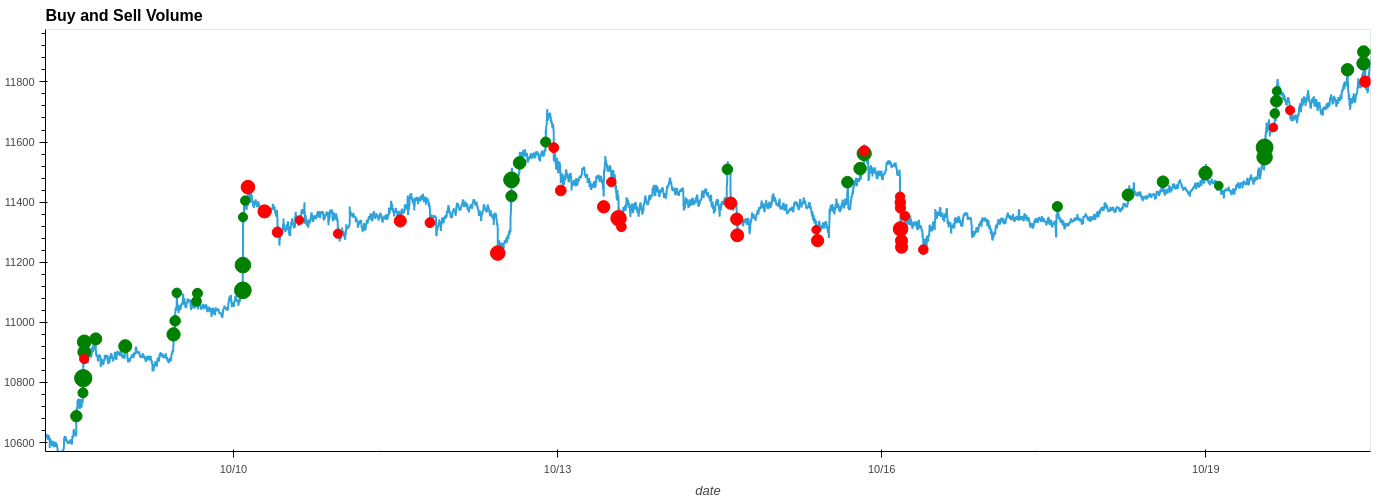
\includegraphics[width=10cm, height = 4cm]{hawkes1.png}
    \caption{An example of buying (green circle) and selling (red circle) volume. The size of the markers, correspond to the amount volume traded.}
    \label{fig:hawkes1}
\end{figure}


At this point, we decided to disregard the mandatory positive counting process and instead use a process that could take negative values. That process would be the difference between positive and negative volumes and it would no longer be a Hawkes process. The first results of our experimentation showed that when the buying side was far greater than the negative selling side, the process would be excited by a positive value and vice versa. Thus, this process could also take negative values, but even if a large negative selling volume appeared, it would take a couple of steps for the function to actually get affected enough and fall below zero (lagging). We consider it natural for sellers to affect buyers and vice versa, and we decided to follow this idea because simple volume self-excitation was not enough.

We used the following custom intensity function: 
\[ \lambda(t|H_t) = \lambda_0(0|H_0) + \sum_{i=1}^{N(t)}(\text{Vol}_{\text{Buy}}(i) - \text{Vol}_{\text{Sell}}(i)) \cdot e^{-\delta(t-T_i)} \]

After modelling the above difference, we used two moving averages, one slow (larger scope) and one faster (smaller window), as above. We then decided to sample based on two different factors, thus creating 4 states. The rationale behind the 4 states, is that we could sample not only when the volume difference spikes, but also when the spike ends, signaling the end of the price action.
The two factors are:
\begin{itemize}
\item Faster MA over slow MA and vice versa (setting a threshold as above)
\item Sign of the difference 
\end{itemize}

And the four states:
\begin{enumerate}
\item Fast moving average of our process would exceed the slow-moving average, indicating there is incoming positive volume (immediate past) at greater rate than the slow-moving average (larger past time window) and the Buyers volume exceeds the Sellers volume.
\item Fast moving average of our process would exceed the slow-moving average, indicating there is incoming positive volume (immediate past) at greater rate than the slow-moving average (larger past time window) and the sellers volume exceed the Buyers volume. We believe this to be a significant indicator for sampling (specifically a shorting the market indicator) because it shows that although there has been a large Buyers rate recently, Sellers appear to significantly take over the reins. Additionaly, it could also indicate the end of an upward price move.
\item Fast moving average of our process would fall below the slow-moving average, indicating there is incoming negative volume (immediate past) at greater rate than the slow-moving average (larger past time window) and the Sellers volume exceeds the Buyers volume.
\item Fast moving average of our process would fall below the slow-moving average, indicating there is incoming negative volume (immediate past) at greater rate than the slow-moving average (larger past time window) but the Buyers volume would exceed the Sellers volume. We also believe this to be a significant indicator for sampling (specifically a longing the market indicator) because it shows that although there has been a large Sellers rate recently, Buyers appear to significantly take over the reins. Additionaly, it could also indicate the end of an downward price move.
\end{enumerate}

In the figure \ref{fig:hawkes2}, we can see an example of the states. Upon carefull inspection of the local minima, we observe increased sell volume (upper graph, red triangle), with the fast MA above the slow one (lower graph, green circle). In many of these occasions, a reversion occurs right away. The latter is a state 2 example. Using the same notion, we distinguish a state 4 example, by observing that at local maxima, the increased buy volume (upper graph, green triangle) is accompanied with the fast MA being under the slow one (lower graph, red cross). In many occasions, a reversion in the price occurs. 

\begin{figure}[H]
	\centering
    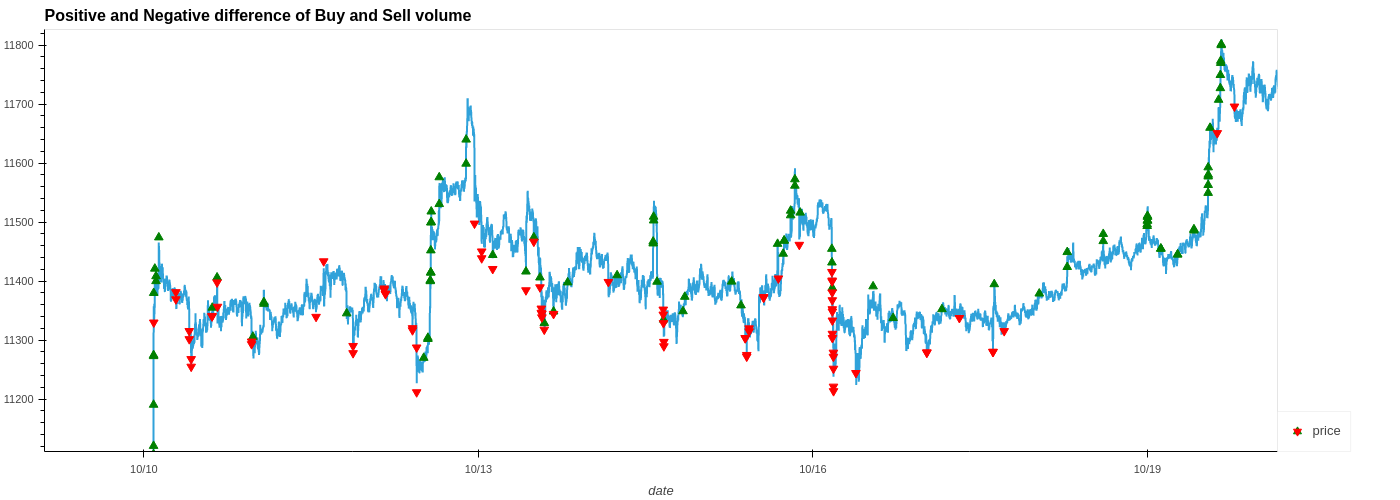
\includegraphics[width=12cm, height = 4cm]{hawkes2.png} \\
    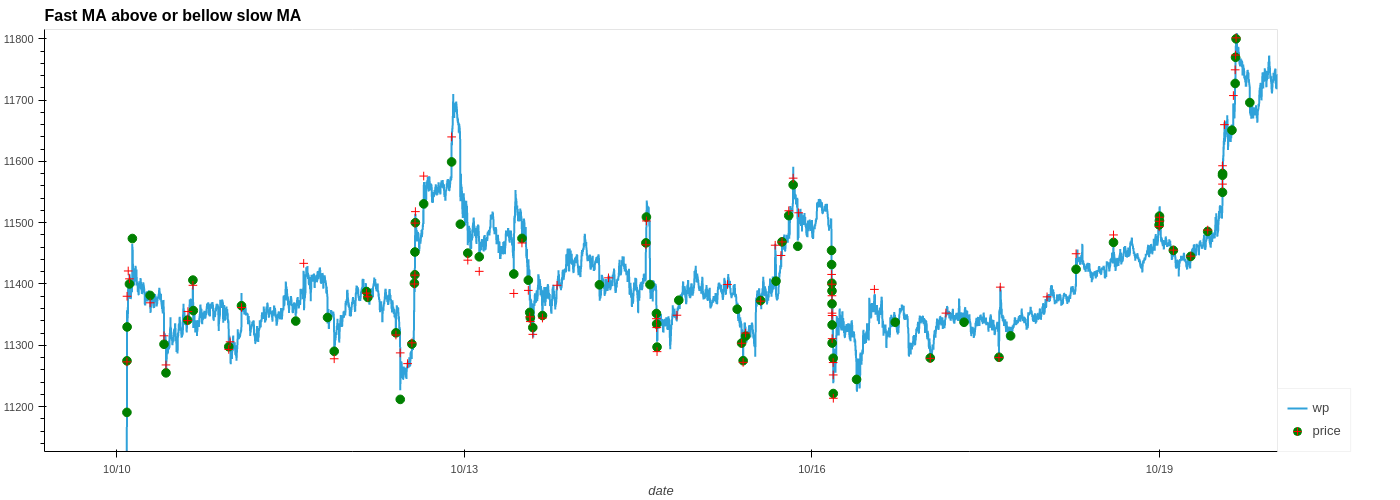
\includegraphics[width=12cm, height = 4cm]{hawkes3.png} \\
	\caption{An illustration of the four states. The first graph corresponds to the first factor and the second graph to the second factor. In the first graph, the green arrows indicate buy volume and the red ones, sell volume. In the second graph, the green circle corresponds to Fast MA > Slow MA, while the red cross, corresponds to the exact opposite.}
    \label{fig:hawkes2}
\end{figure}


The reader should keep in mind, that the sampling took place in the 'second' timeframe, while the price in the figure above, is plotted from the 'minute' timeframe, using the mean price during that minute. Therefore, the real volatility cannot be grasped by this graph, and some points seem to wander off the price plot. In order to bypass that shortcoming, and furthermore, to illustrate visually how modelling - sampling - parameters look like, a zoom-in figure, with price displayed in seconds will be presented.


\begin{figure}[H]
	\centering
    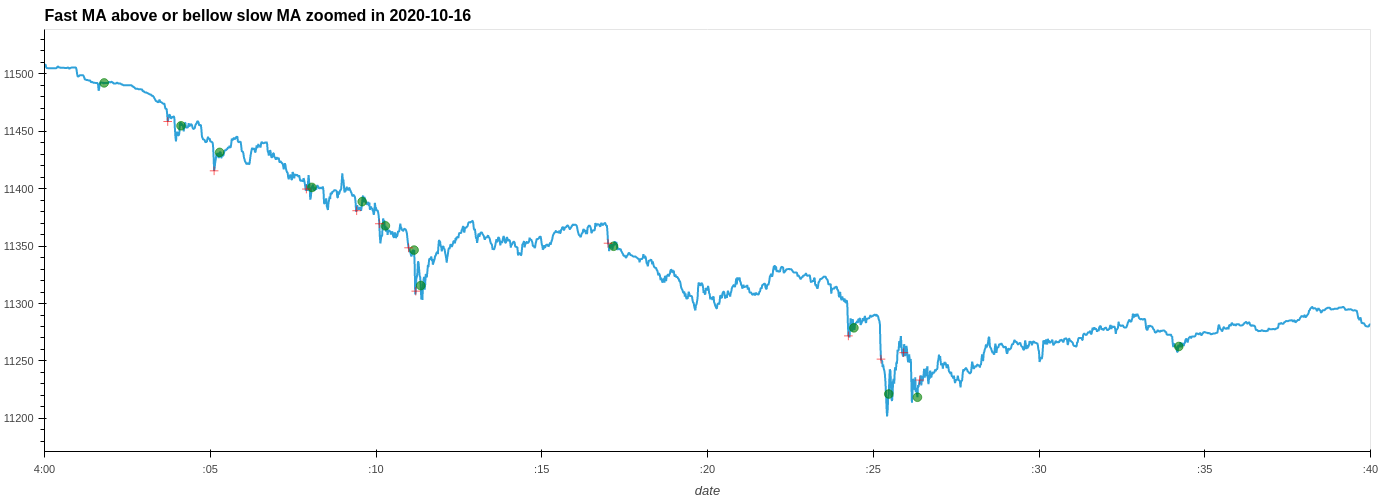
\includegraphics[width=12cm, height = 4cm]{hawkeszoom1.png} \\
    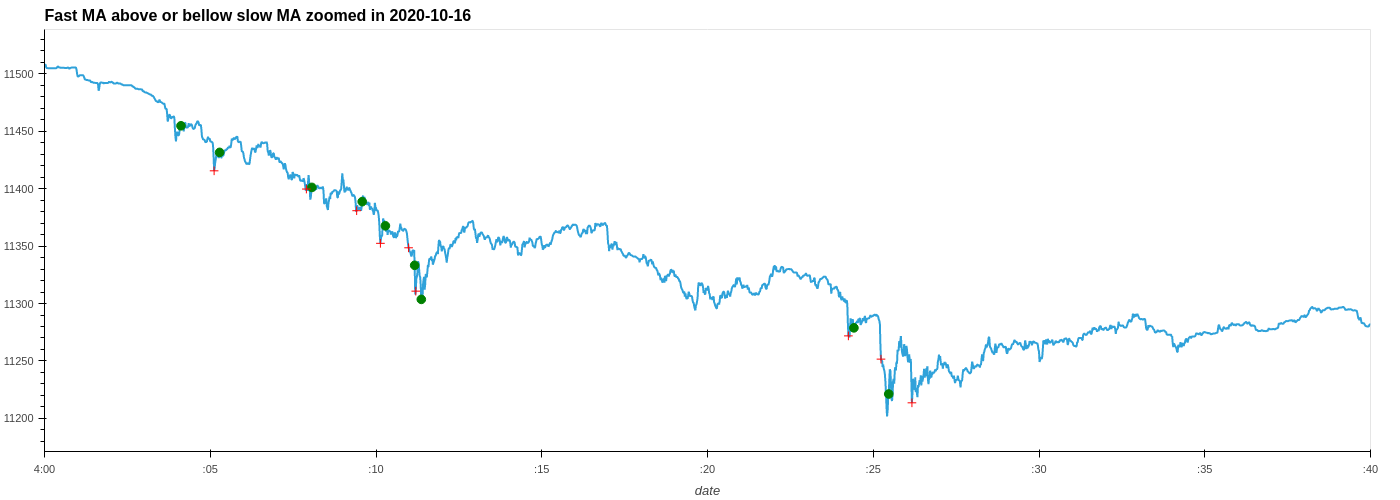
\includegraphics[width=12cm, height = 4cm]{hawkeszoom2.png} \\
    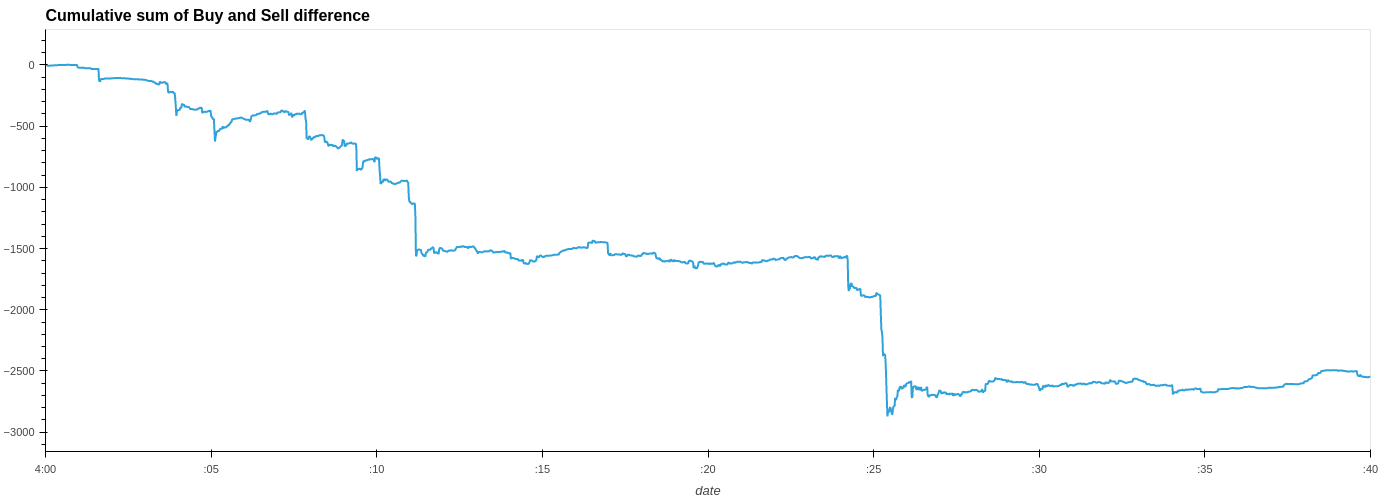
\includegraphics[width=12cm, height = 4cm]{hawkeszoom3.png} \\
    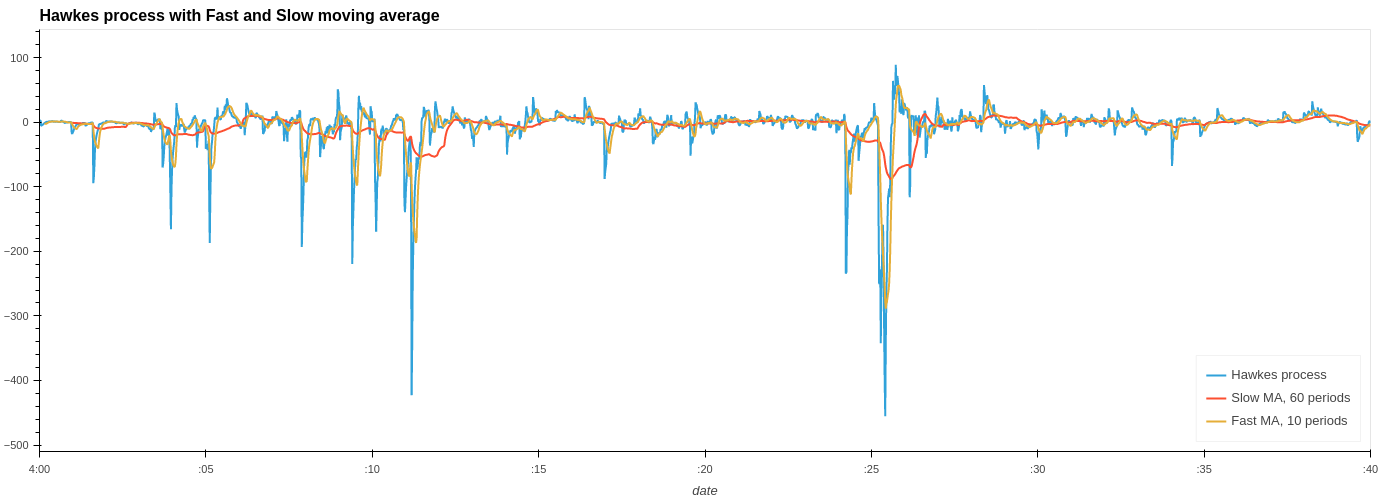
\includegraphics[width=12cm, height = 4cm]{hawkeszoom4.png}
	\caption{Several plots of a 'Hawkes process' on the difference of buy and sell volume along with an example of sampling using moving averages on the above process (in 'seconds' timeframe).}
    \label{fig:hawkeszoom}
\end{figure}


In 2020-10-16 from 04:00 to 04:40, there was a rapid correction in BTCUSD(T) pair. The figure \ref{fig:hawkeszoom}, presents the 'Hawkes process' on the buy and sell volume difference, and then a sampling effort on this process. At first, the third plot (Cumulative sum of Buy and Sell difference), shows that the sell volume is greater than the buy volume. There are also some points where the sell pressure is higher and periods where buy and sell volume are approximately the same. We observe that in the points where imbalance between buy and sell volume occurs, the 'Hawkes process' spikes and then returns at the mean level (which was set at zero). 

The Fast MA (10 periods - orange colour) and Slow MA (60 periods - red colour), cross each other and produce the green circle and red cross of the second plot (Fast MA above or bellow slow MA). The rationale behind this sampling, is that when a falling fast MA crosses a falling slow MA, the price falls (and vice verca), and thus a red arrow of the first plot is accompanied with a red cross of the second plot. Since the 'first point sampled' represents the beginning of one move, the next point that must be sampled, should signify the end of it, where a rising fast MA crosses a falling slow MA. This way, we can sample the beginning (or close to beginning) and the end of the move. Nevertheless, if the price begins to fall gradualy, with no major spikes on the 'Hawkes process', and the fast and slow MA slowly converge, there would be no sampling. Furthermore, this way of sampling is very sensitive to the parameters chosen (fast and slow MA) and as we can see in the second and fourth plot of figure \ref{fig:hawkeszoom}, there are times that the fast is not fast enough to catch the very fast price moves, but does a better job in sampling correctly the larger moves along with their ending.

\subsubsection{Positive and Negative Volume}


From a market microstructure perspective, the search of imbalances of signed volumes (positive volume and negative volume), could reveal the presence of information \cite{marcos}. Based on the work of de Prado, a more precise way of sampling, is to sample when imbalances become apparent in the market. These imbalances could be seen as new information. At this point we need to be precise as to what we will mean from now on, when the word 'imbalance' is used: deviation of a feature, from our expectation that is calculated from the immediate past of the feature (short or long past depending on the parameters chosen). Soon after the imbalance occurs, a new expectation is created that gets updated, as new data arrive.

The 'Hawkes process' of the previous subsection, is used in order to sample the imbalances on the difference between buy and sell volume. A very similar way of sampling will be attempted here as well, by changing the 'buy' and 'sell' with 'positive' and 'negative'. We begin by calculating the sign \(b_t\) of returns \(r_t\):
\[ 
b_t =
\begin{cases}
b_{t-1} \text{ for } r_t = 0 \\
\text{sign}(r_t) \text{ for } r_t \neq 0
\end{cases}
\]

The above calculation results to an array with \(\{1,-1\}\), depending on the sign of the returns. Lets denote with \( v_t \) an array that corresponds to the tick by tick volume, and also keep in mind that those arrays get updated as new data arrive. By multiplying the two arrays row by row (Hadamard product), the array created, has the same values as \( v_t \) but signed as positive or negative based on the returns. This array will be used in order to sample any imbalances found to the positive or to the negative side. One way to do the sampling is the proposed by de Prado way, where 
\[ \theta_T = \max(\sum_{t = t_0}^{T} b_tv_t) \]
represents the imbalance on a non fixed interval of length, \(T\) number of ticks. Then the expectation of the next imbalance \( \mathbb{E}_0(\theta_T) \) is computed using the expectation of the next bars length \( \mathbb{E}_0(T) \) using the next formula:
\[ \mathbb{E}_0(\theta_T) = \mathbb{E}_0(T) \max\{P[b_t=1]\mathbb{E}_0[v_t|b_t=1], (1-P[b_t=1])\mathbb{E}_0[v_t|b_t=-1]\} \]

The above way of sampling is called \textit{Volume Runs Bars} \cite{marcos}. Basically, we will sample the imbalances of summed signed volumes. A first thought is to sample when these imbalances cross a fixed threshold. This way, we might be able to sample correctly during 'normal' volume, but at times of high (low) volume we will oversample (undersample). 

In order to overcome the fixed threshold problem, we will use a fast exponential moving average (EWMA) and a slow EWMA, which actually serves as a dynamically changing threshold. The sampling will take place, when the fast EWMA crosses the slow EWMA. The EWMA, is a type of moving average, which keeps all past information with decaying weights:
\[ \text{EWMA}_t = \alpha \cdot x_t + (1 - \alpha) \cdot \text{EWMA}_{t-1} \]
 where \(x_t\) is the value of the variable at time \(t\) and \(\alpha\) controls the importance of the recent value vs the old ones \cite{prod}. A slow EWMA has a small \(alpha\) in order to resist temporary fluctuations, but at the same time, account for them when EWMA of time \(T > t\) is calculated. The fast EWMA on the other hand, has a bigger \(\alpha\), chosen in order to prioritize the  very recent history. An example of this sampling, can be seen on the figure bellow.


\begin{figure}[H]
	\centering
    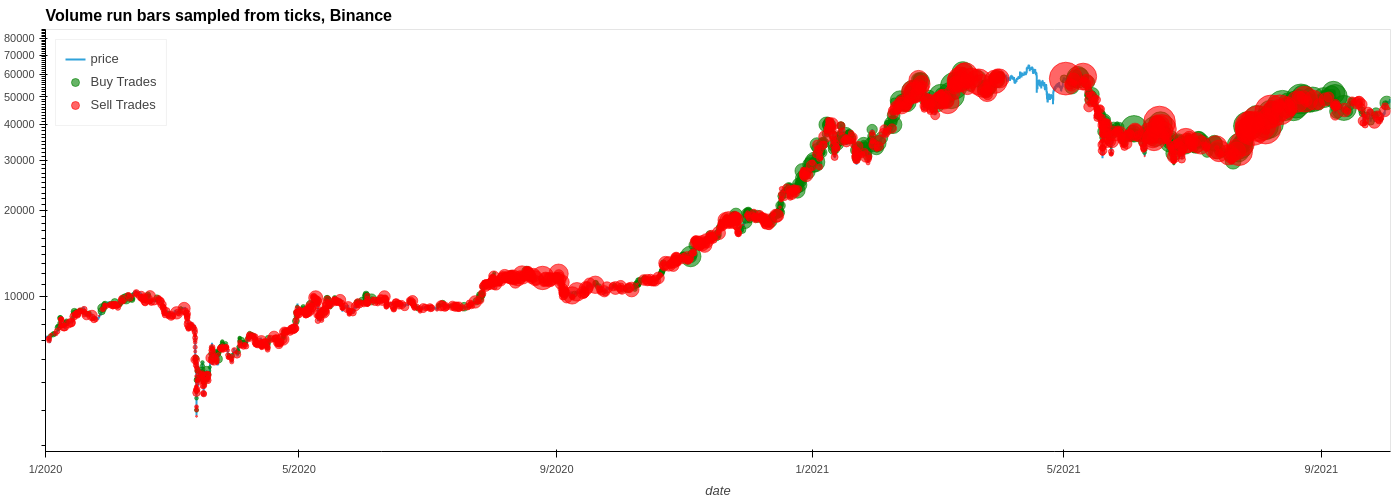
\includegraphics[width=12cm, height = 4cm]{vol_run_bin1.png} \\
    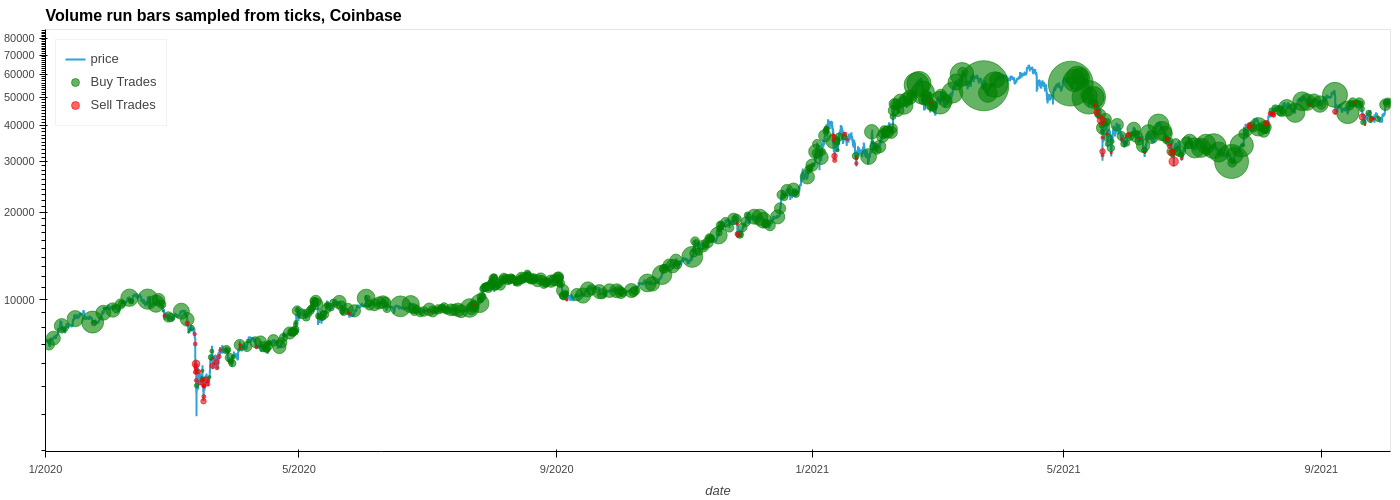
\includegraphics[width=12cm, height = 4cm]{vol_run_coi1.png}
	\caption{An example of volume runs bars, sampled from ticks, for Coinbase and Binance.}
    \label{fig:vol_run}
\end{figure}

In figure \ref{fig:vol_run}, the green circles represent positive volume, and the red ones, negative volume. Visually the sampling seems to be as expected, since the positive volume is mainly found when the price is rising and the negative, when the price is falling. Furthermore, based on the parameters of the EWMA used in each exchange (Binance and Coinbase), we can see slightly different sampling.

Elaborating on the above effort, we can sample the difference of positive and negative volumes from buy-only and sell-only trades. The rationale behind this decision, is to sample when negative volume, which corresponds to negative returns and subsequently to a falling price (even if very short term), is associated with buy-side trades, and vice versa. Additionaly, for experimenting purposes, we will sample the difference of buy and sell volume from positive and negative only trades, in order to capture the sell (buy) volume on positive (negative) price moves.

For simplicity purposes, we will sample from 'second' timeframe and not directly from tick data. At first we will construct four new columns for each exchange:

\begin{enumerate}
\item Positive volume with buying orders
\item Positive volume with selling orders
\item Negative volume with buying orders
\item Negative volume with selling orders
\end{enumerate}

After resampling all exchanges to the 'second' timeframe, the newly created columns, are summed row wise for all exchanges. Using these columns, we construct 4 new ones, by simply subtracting one from the other:

\begin{enumerate}
\item Positive volume: Buying volume - Selling volume
\item Negative volume: Buying volume - Selling volume
\item Buying volume: Positive volume - Negative volume
\item Selling volume: Positive volume - Negative volume
\end{enumerate}

The green (red) colour will be used to indicate positive (negative) volume while a triangle (inverted triangle) for buy (sell) volume. In figure \ref{fig:pos_neg}, upper graph, we can see the \(\text{Vol}_{Buy} - \text{Vol}_{Sell} \), when \(\text{Vol}_{Sell} > \text{Vol}_{Buy} \) under positive volume (returns). 
 
\begin{figure}[H]
	\centering
    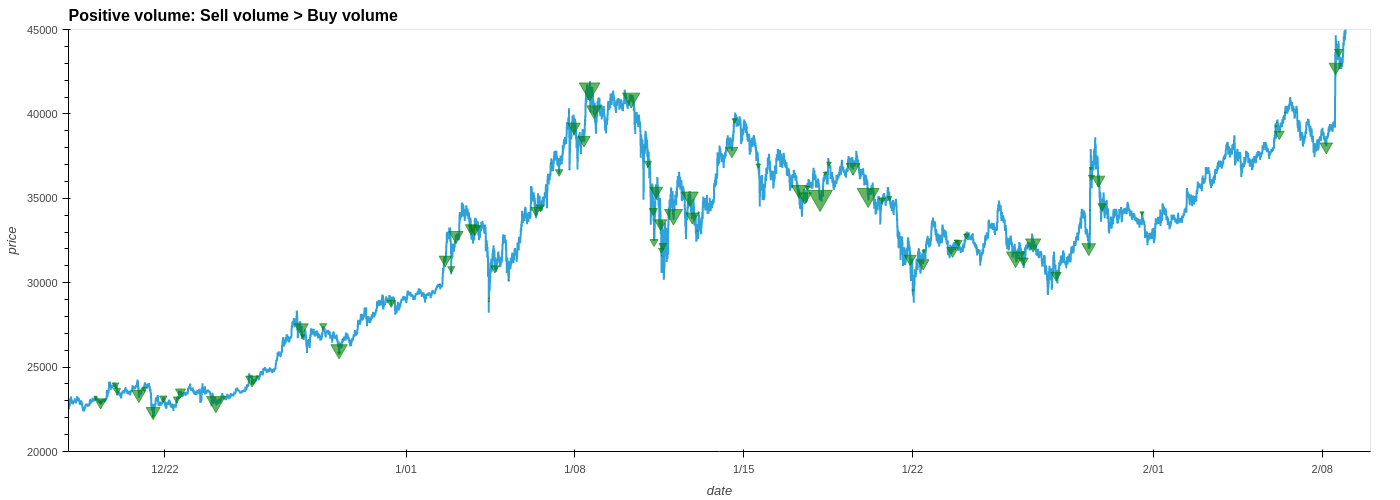
\includegraphics[width=12cm, height = 4cm]{pos1.png} \\
    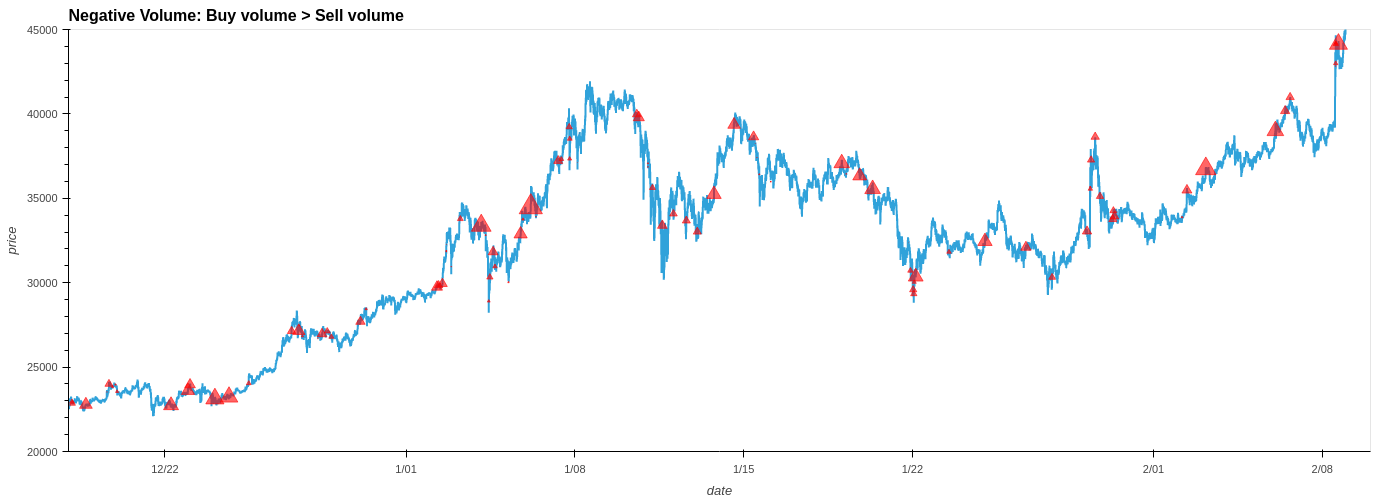
\includegraphics[width=12cm, height = 4cm]{neg1.png}
	\caption{Buying - Selling volume imbalance on positive and negative only volume.}
    \label{fig:pos_neg}
\end{figure}

What we expect to extract from the above sampling, is the occasions where selling volume spikes during positive returns, signaling thus a short term price reversal. Similarly, in the second graph \ref{fig:pos_neg}, we sample buying volume spikes, during negative returns (or potentialy a falling price). Again, we expect to find a short term reversal, since buying activity should stop or slow down negative returns or a falling price.

Similarly, given the buy volume, we sample the difference  \(\text{Vol}_{Positive} - \text{Vol}_{Negative} \), when \(\text{Vol}_{Negative} > \text{Vol}_{Positive} \), see figure \ref{fig:buy_sell}, upper graph. On the second graph, we can see the excess of positive volume, under sell trades.

This market behavior seems unintuitive. The volume that is computed in this sampling, represents the majority of volume traded in BTCUSD(T) markets. If we assume, that there is no significant volume in another exchange, the rising price with sell trades and falling price with buy trades, should be significant.

\begin{figure}[H]
	\centering
    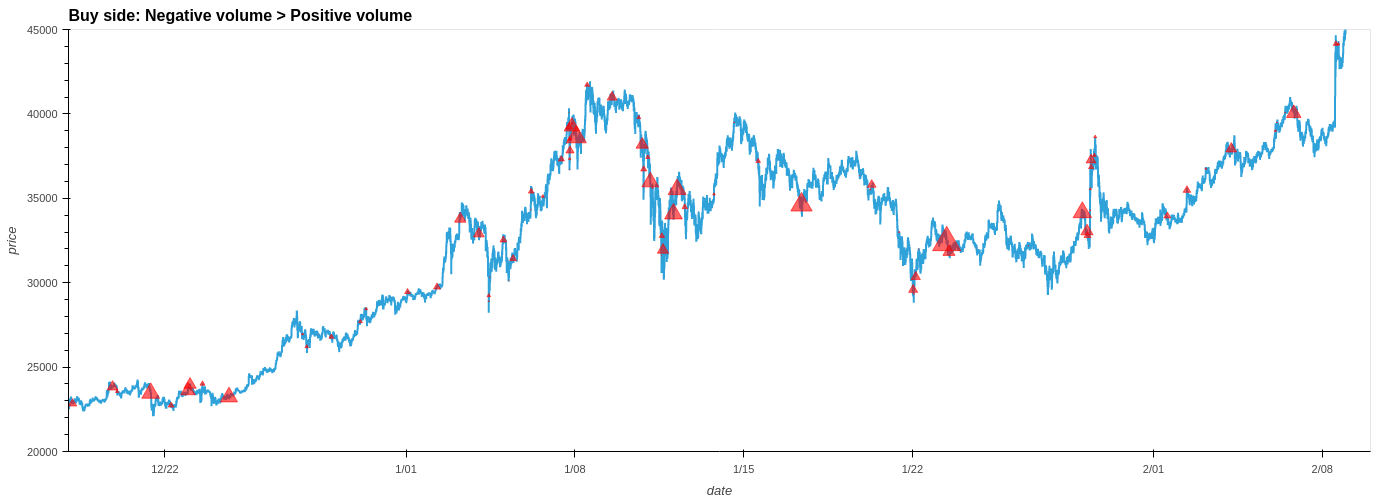
\includegraphics[width=12cm, height = 4cm]{buy1.png} \\
    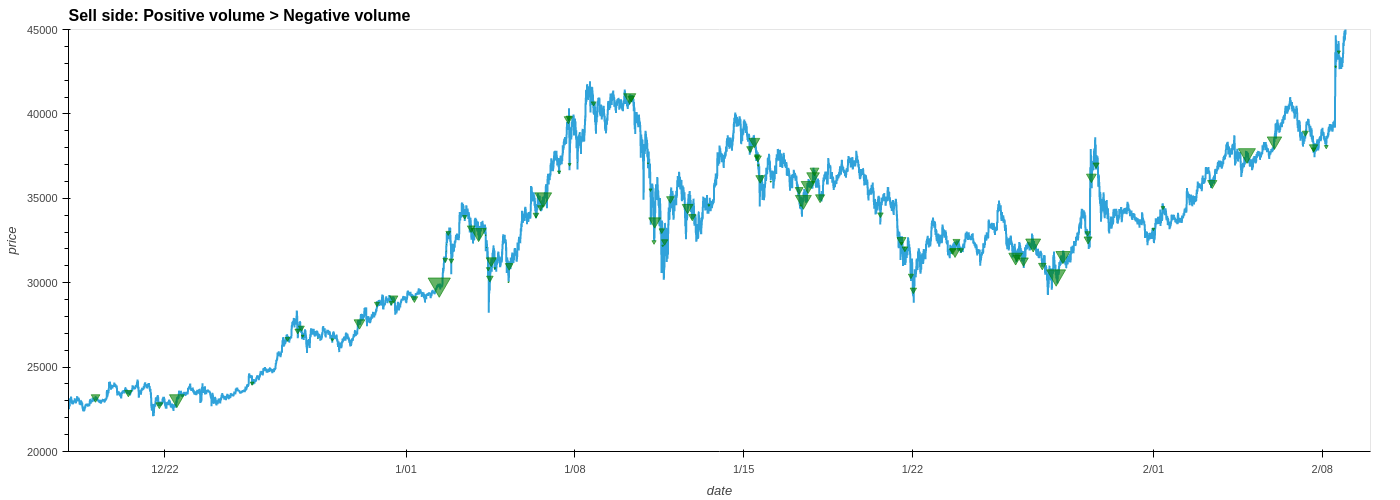
\includegraphics[width=12cm, height = 4cm]{sell1.png}
	\caption{Positive - Negative volume imbalance on buy and sell only trades.}
    \label{fig:buy_sell}
\end{figure}


\section{Speed of the market}

We define the 'speed of the market' to be the rate of incoming trades. Since the trades arrive in an asynchronous way, the \texttt{TimeDelta} between two consecutive trades, vary over time. There will be occasions when the \texttt{TimeDelta} contracts and others when it expands. We are interested in those times where it remains contracted for a 'sufficient' number of trades, and as above, the threshold for what is 'sufficient', will dynamically change.

The \texttt{DateTime} column of our dataset, is sampled from milliseconds (1 second = 1,000 milliseconds). After been transformed to \texttt{Unix} time, we are left with an array of 11 digits integers. The high volume - high transaction rates exchanges, (Binance, Coinbase, Huobi) exhibit many transactions that occur at the same millisecond. That could be an indication of high frequency trading, or iceberg orders. 

We transform the \texttt{DateTime} array in the following way: at first we compute the first difference in order to calculate the \texttt{TimeDelta}. Then we replace the zeroes (trades that occured the same millisecond) with a number \(z\) such that \( 0 < z < 1 \). The resulting array \texttt{dt}, contains integers as \texttt{TimeDelta} between trades that occured in different time, and a float \(z\), for trades that happened the exact same time. Lastly, we compute \texttt{speed} as:
\[ \texttt{speed} = \frac{1}{\texttt{dt}} \] 

The resulting array \texttt{speed} contains floats \( < 1 \) everywhere except for the trades that happened the same time, where the values are \( > 1 \). At times, when there are few trades or no trades per (milli) second, the \texttt{speed} takes values, \( < \frac{1}{100000} \). When trades though occur at the same time, the \texttt{speed} spikes become pronounced. In order to sample, we will create the cumulative sums of the \texttt{speed}. If transaction rates are steady, there will be no sample. Conversely, if they change rapidly, an imbalance will transpire in the form of a spike, and thus, that point will be sampled.

By slicing the Coinbase dataset, from \texttt{2020-12-18 00:00:01.086} to \texttt{2021-02-10 23:59:59.700}, we compute the \texttt{TimeDelta} between the two dates in milliseconds: \( 4,751,998,614 \). If the arrival of trades were uniformly distributed, we would expect one trade every approximately \( 295 \) milliseconds.

\begin{figure}[H]
	\centering
    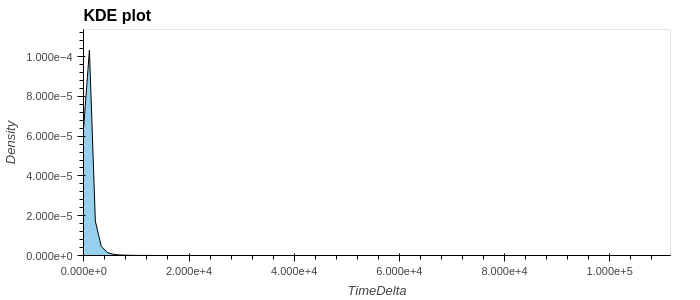
\includegraphics[width=10cm, height = 4cm]{kde_time.png}
	\caption{KDE plot of timedeltas between consecutive trades, Coinbase.}
    \label{fig:kde_time}
\end{figure}

As we can see in figure \ref{fig:kde_time}, the \texttt{TimeDeltas} are not normally distributed while the proposed distributions to model trade arrival times, are the Exponential and the Weibull \cite{weib}. In the above dataset, the \(28.57\%\) of the trades, are executed at the same millisecond while the \(38.34\%\), are less than \(295.769\) milliseconds (\(0.295\) seconds) away. By clustering the trades that were recorded on the same millisecond, we find that the mean amount of volume of these clusters were \( 0.32 \) btc, while there were significant clusters with more than 50 btc each.

A characteristic of these clusters, is that the entire volume that was traded whithin the millisecond, was either buying or selling. Furthermore, note, that the 'same millisecond' trades, which account for the \(28.57\%\) of all trades, control approximately \(44.23\%\) of total volume traded. We conclude that these trades should be sampled carefully, with buying and/or selling volume in mind, positive and/or negative volume, and the effect of these trades in the returns as well.

In the figure bellow \ref{fig:speed_coi}, we showcase an example of sampling with respect to the speed, for the market of Coinbase. The algorithm used to sample the imbalances with regard to speed, is the same as in positive-negative volume sampling. That means, that each imbalance is recorded, and the bar created, consists of all information aggregated between the two samples, while no further information is given on the 'millisecond' trades.

\begin{figure}[H]
	\centering
    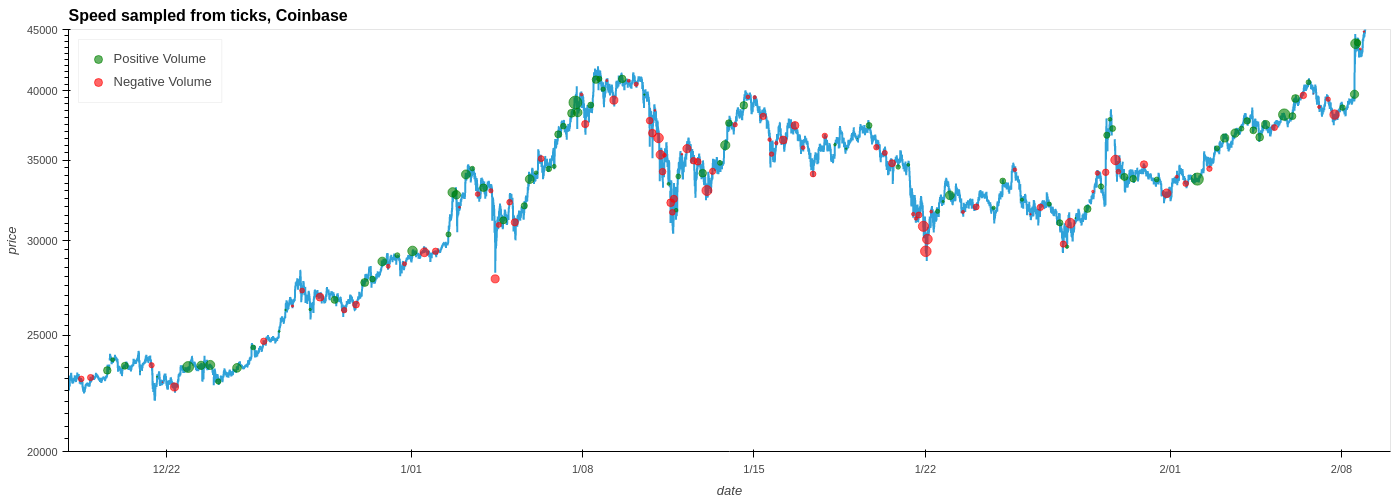
\includegraphics[width=12cm, height = 4cm]{speed_coi1.png} \\
    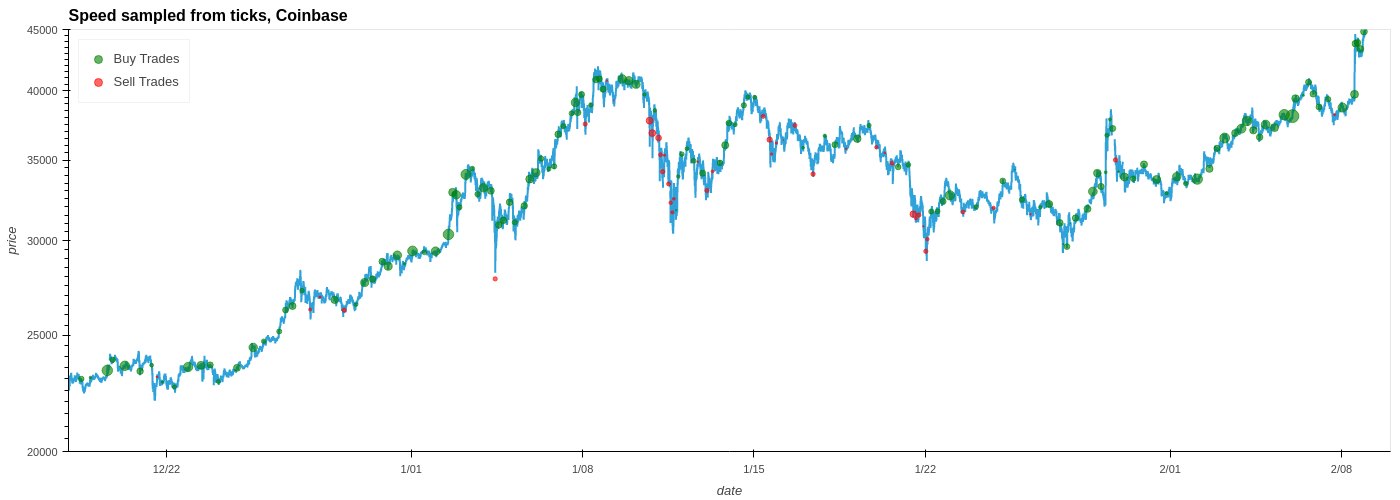
\includegraphics[width=12cm, height = 4cm]{speed_coi2.png}
	\caption{Speed sampled from a subset of Coinbase. The area of the circles displayed above, were calculated by aggregating the volume with respect to the sign (positive-negative) or to the side that initiated the trade (buying-selling), between two consecutive samples.}
    \label{fig:speed_coi}
\end{figure}

By further enhancing the above sampling, we will extract all milliseconds that 'contain' more than one trade, and sample only on these trades, assuming that they were executed from informed traders. In order to create the figure bellow \ref{fig:milli1}, the 'millisecond trades' were extracted and aggregated into one sample each (all trades of the same millisecond, aggregated to one trade), keeping the difference of buy-sell volume, positive-negative volume, number of trades and cumulative returns (\texttt{cumprod}). Out of the new dataset, the \(2500\) samples (out of approximately \(2,000,000\)) with the most trades, were plotted. The graph bellow, is a zoom-in on the actual plot.

\begin{figure}[H]
	\centering
    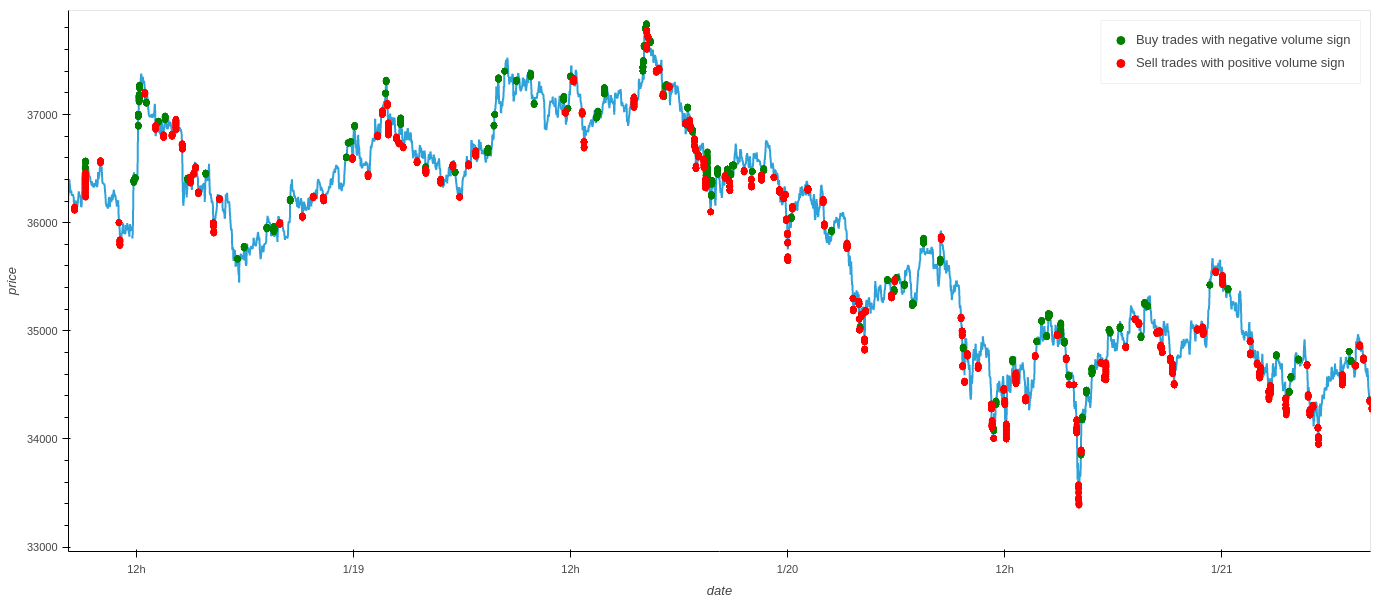
\includegraphics[width=12cm, height = 4cm]{milli1.png}
	\caption{Each circle represents one sample that actually contains several trades. The samples shown here, are selected to contain the largest number of trades.}
    \label{fig:milli1}
\end{figure}



\section{PCA Sampling}

The term \textit{PCA Sampling}, refers to sampling, when all exchanges converge in a specific behavior. That behavior could be a rising volume, increased rate of transactions, increased buying or selling volume etc. In this sampling, it is assumed that all exchanges are of 'equal' importance, even though different sampling for USDT and USD markets, is presented as well. The rationale behind this idea, is that similar activity on all exchanges, should be indicative of identical information across the market.

The figure bellow \ref{fig:pca_sampl1}, illustrates a simple PCA sampling effort. The sampling took place on the 'minute' timeframe of positive volume (green circle) and negative volume (red circle). A PCA analysis (with covariance matrix) is applied every \(200\) minutes in an overlapping manner, and a sample is taken if the explained variance ratio of the 1st principal component, is greater than \(0.9\). The same could be applied on buying/selling volume, speed of the market, high speed trades (the 'millisecond' iceberg trades from previous section) and generally, on meaningful subsets or transformations of the dataset.

 
\begin{figure}[H]
	\centering
    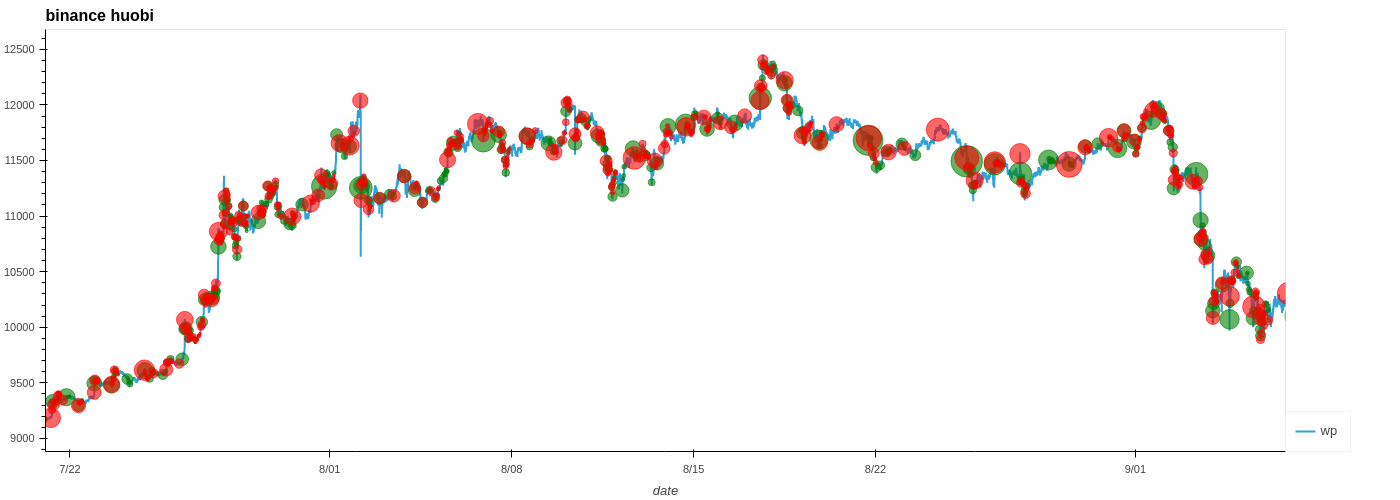
\includegraphics[width=12cm, height = 4cm]{pca_sampl1.png} \\
    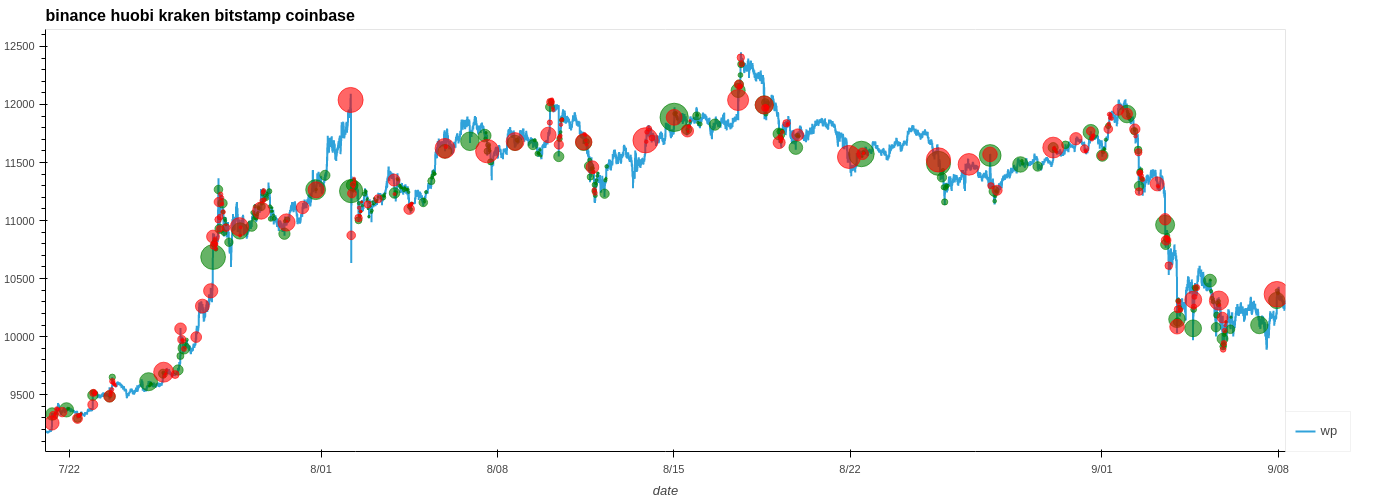
\includegraphics[width=12cm, height = 4cm]{pca_sampl2.png} \\
    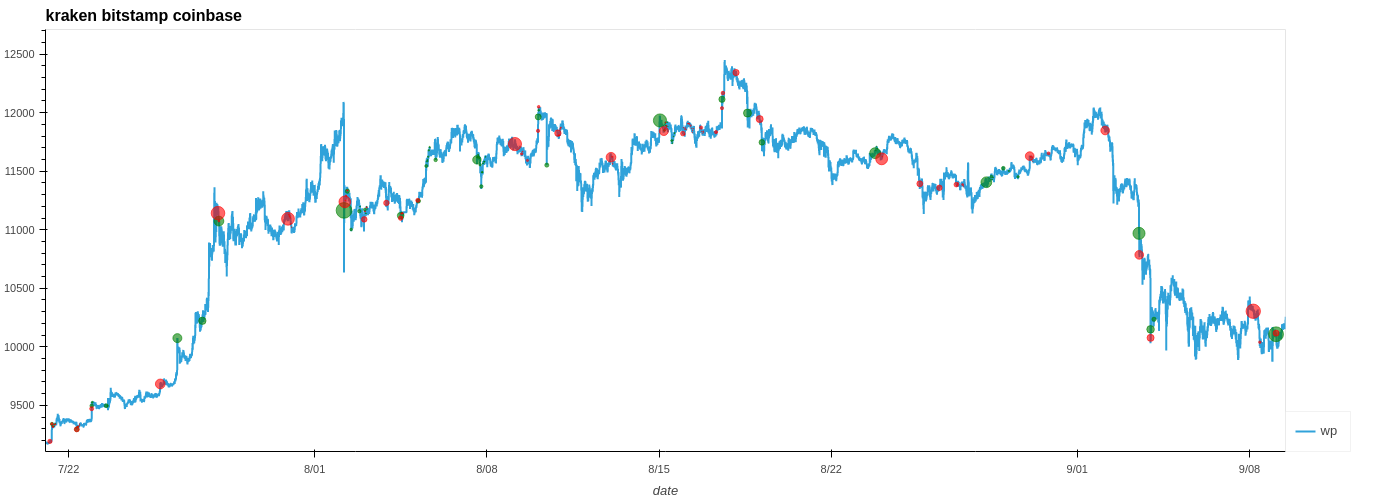
\includegraphics[width=12cm, height = 4cm]{pca_sampl3.png}
	\caption{An example of PCA sampling on USD, USDT and combined markets on positive/negative volume.}
    \label{fig:pca_sampl1}
\end{figure}

The first thing to notice, is that under the same parameters, the algorithm sampled more frequently on the USDT market. On the other hand, on the USD market, it seems to undersample, since there are fewer times when the 1st PC was greater than \(0.9\). The combined market, shows a different picture from the USDT (and the USD) market and even after adjusting the parameters in a way to sample approximately the same number of points in both occasions, the sampling was different enough, to justify both sampling efforts in one's arsenal.

We repeat the same thing as above but this time on buying and selling volume (see figure \ref{fig:pca_sampl2}). The parameters remain the same (window for PCA = \(200\) minutes, threshold to sample is 1st PC > \(0.9\)). By contrasting the binance-huobi graph from above with the one from bellow, we observe that the algorithm sampled positive volume with selling activity and vice verca in many cases. That creates an hypothesis to be tested, as to whether this pattern is to be found mostly in local maxima and minima.



\begin{figure}[H]
	\centering
    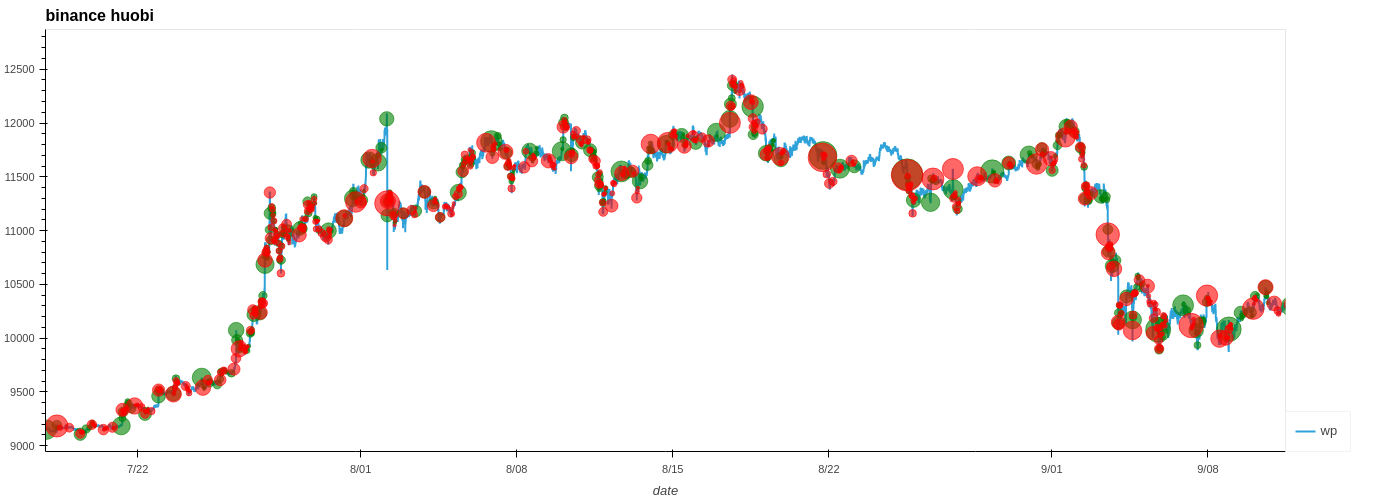
\includegraphics[width=12cm, height = 4cm]{pca_sampl4.png} \\
    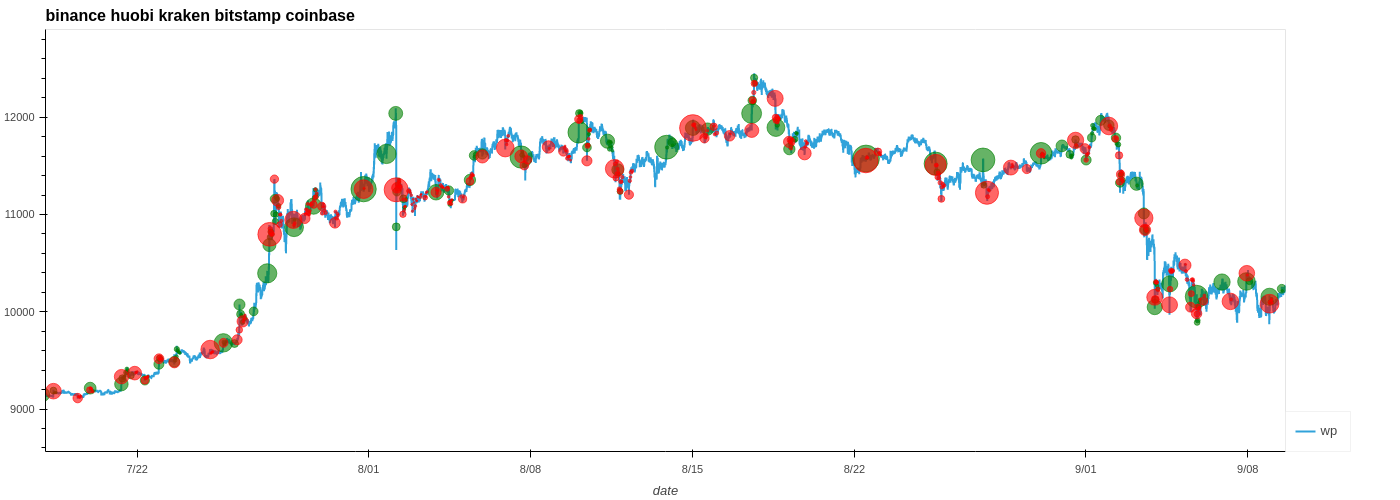
\includegraphics[width=12cm, height = 4cm]{pca_sampl5.png} \\
    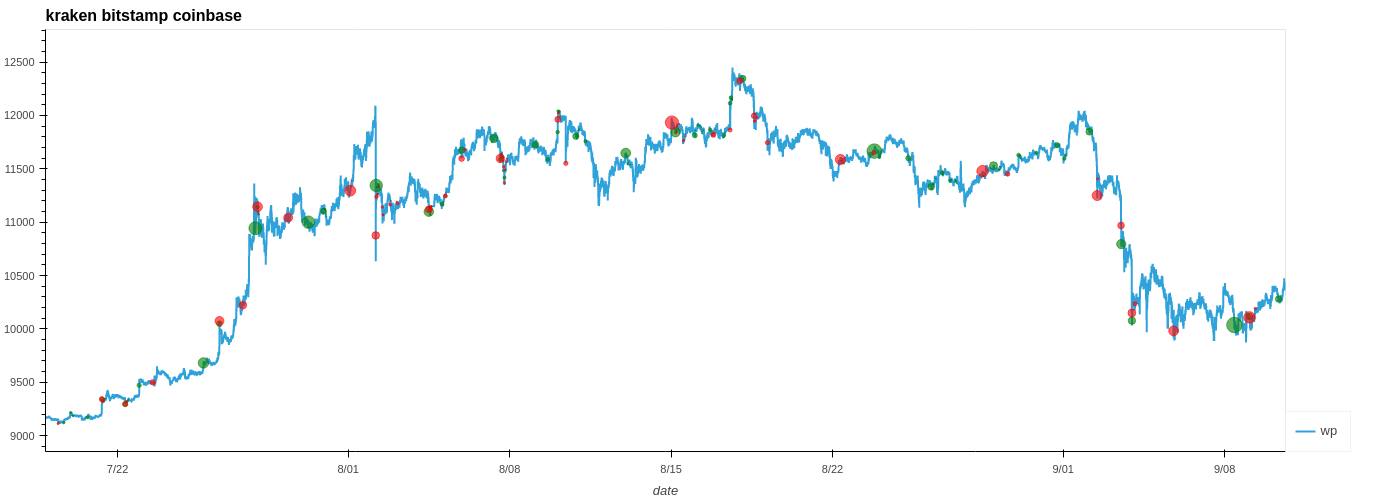
\includegraphics[width=12cm, height = 4cm]{pca_sampl6.png}
	\caption{An example of PCA sampling on USD, USDT and combined markets on buying/selling volume.}
    \label{fig:pca_sampl2}
\end{figure}


